%Version 3.1 December 2024
% See section 11 of the User Manual for version history
%
%%%%%%%%%%%%%%%%%%%%%%%%%%%%%%%%%%%%%%%%%%%%%%%%%%%%%%%%%%%%%%%%%%%%%%
%%                                                                 %%
%% Please do not use \input{...} to include other tex files.       %%
%% Submit your LaTeX manuscript as one .tex document.              %%
%%                                                                 %%
%% All additional figures and files should be attached             %%
%% separately and not embedded in the \TeX\ document itself.       %%
%%                                                                 %%
%%%%%%%%%%%%%%%%%%%%%%%%%%%%%%%%%%%%%%%%%%%%%%%%%%%%%%%%%%%%%%%%%%%%%

%%\documentclass[referee,sn-basic]{sn-jnl}% referee option is meant for double line spacing

%%=======================================================%%
%% to print line numbers in the margin use lineno option %%
%%=======================================================%%

% FOR NATURE JOURNAL SUBMISSION
\documentclass[pdflatex,sn-nature]{sn-jnl}% Style for submissions to Nature Portfolio journals

%%=========================================================================================%%
%% the documentclass is set to pdflatex as default. You can delete it if not appropriate.  %%
%%=========================================================================================%%

%\documentclass[sn-basic, twocolumn]{sn-jnl}% Basic Springer Nature Reference Style/Chemistry Reference Style

%%Note: the following reference styles support Namedate and Numbered referencing. By default the style follows the most common style. To switch between the options you can add or remove Numbered in the optional parenthesis. 
%%The option is available for: sn-basic.bst, sn-chicago.bst%  
 
%%\documentclass[pdflatex,sn-nature]{sn-jnl}% Style for submissions to Nature Portfolio journals
%%\documentclass[pdflatex,sn-basic]{sn-jnl}% Basic Springer Nature Reference Style/Chemistry Reference Style
%%\documentclass[pdflatex,sn-mathphys-num]{sn-jnl}% Math and Physical Sciences Numbered Reference Style
%%\documentclass[pdflatex,sn-mathphys-ay]{sn-jnl}% Math and Physical Sciences Author Year Reference Style
%%\documentclass[pdflatex,sn-aps]{sn-jnl}% American Physical Society (APS) Reference Style
%%\documentclass[pdflatex,sn-vancouver-num]{sn-jnl}% Vancouver Numbered Reference Style
%%\documentclass[pdflatex,sn-vancouver-ay]{sn-jnl}% Vancouver Author Year Reference Style
%%\documentclass[pdflatex,sn-apa]{sn-jnl}% APA Reference Style
%%\documentclass[pdflatex,sn-chicago]{sn-jnl}% Chicago-based Humanities Reference Style

%%%% Standard Packages
%%<additional latex packages if required can be included here>

\usepackage{graphicx}%
\usepackage{multirow}%
\usepackage{amsmath,amssymb,amsfonts}%
\usepackage{amsthm}%
\usepackage{mathrsfs}%
\usepackage[title]{appendix}%
\usepackage{xcolor}%
\usepackage{textcomp}%
\usepackage{manyfoot}%
\usepackage{booktabs}%
\usepackage{algorithm}%
\usepackage{algorithmicx}%
\usepackage{algpseudocode}%
\usepackage{listings}%
%%%%

%%%%%=============================================================================%%%%
%%%%  Remarks: This template is provided to aid authors with the preparation
%%%%  of original research articles intended for submission to journals published 
%%%%  by Springer Nature. The guidance has been prepared in partnership with 
%%%%  production teams to conform to Springer Nature technical requirements. 
%%%%  Editorial and presentation requirements differ among journal portfolios and 
%%%%  research disciplines. You may find sections in this template are irrelevant 
%%%%  to your work and are empowered to omit any such section if allowed by the 
%%%%  journal you intend to submit to. The submission guidelines and policies 
%%%%  of the journal take precedence. A detailed User Manual is available in the 
%%%%  template package for technical guidance.
%%%%%=============================================================================%%%%

%% as per the requirement new theorem styles can be included as shown below
\theoremstyle{thmstyleone}%
\newtheorem{theorem}{Theorem}%  meant for continuous numbers
%%\newtheorem{theorem}{Theorem}[section]% meant for sectionwise numbers
%% optional argument [theorem] produces theorem numbering sequence instead of independent numbers for Proposition
\newtheorem{proposition}[theorem]{Proposition}% 
%%\newtheorem{proposition}{Proposition}% to get separate numbers for theorem and proposition etc.

\theoremstyle{thmstyletwo}%
\newtheorem{example}{Example}%
\newtheorem{remark}{Remark}%

\theoremstyle{thmstylethree}%
\newtheorem{definition}{Definition}%

\raggedbottom
%%\unnumbered% uncomment this for unnumbered level heads

\begin{document}

\title[Gender Similarities Dominate Mathematical Cognition at the Neural Level: A Japanese fMRI Study Using Advanced Wavelet Analysis and Generative AI]{Gender Similarities Dominate Mathematical Cognition at the Neural Level: A Japanese fMRI Study Using Advanced Wavelet Analysis and Generative AI}

%%=============================================================%%
%% GivenName	-> \fnm{Joergen W.}
%% Particle	-> \spfx{van der} -> surname prefix
%% FamilyName	-> \sur{Ploeg}
%% Suffix	-> \sfx{IV}
%% \author*[1,2]{\fnm{Joergen W.} \spfx{van der} \sur{Ploeg} 
%%  \sfx{IV}}\email{iauthor@gmail.com}
%%=============================================================%%

\author{\fnm{Tatsuru} \sur{Kikuchi}}\email{tatsuru.kikuchi@e.u-tokyo.ac.jp}

%\author[2,3]{\fnm{Second} \sur{Author}}\email{iiauthor@gmail.com}
%\equalcont{These authors contributed equally to this work.}

%\author[1,2]{\fnm{Third} \sur{Author}}\email{iiiauthor@gmail.com}
%\equalcont{These authors contributed equally to this work.}

\affil{\orgdiv{Faculty of Economics}, \orgname{The University of Tokyo}, \orgaddress{\street{7-3-1 Hongo}, \city{Bunkyo-ku}, \postcode{113 0033}, \state{Tokyo}, \country{Japan}}}

%\affil[2]{\orgdiv{Department}, \orgname{Organization}, \orgaddress{\street{Street}, \city{City}, \postcode{10587}, \state{State}, \country{Country}}}

%\affil[3]{\orgdiv{Department}, \orgname{Organization}, \orgaddress{\street{Street}, \city{City}, \postcode{610101}, \state{State}, \country{Country}}}

%%==================================%%
%% Sample for unstructured abstract %%
%%==================================%%

\abstract{Recent large-scale behavioral studies suggest early emergence of gender differences in mathematical performance within months of school entry. However, these findings lack direct neural evidence and are constrained by cultural contexts. We conducted functional magnetic resonance imaging (fMRI) during mathematical tasks in Japanese participants (N = 156), employing an advanced wavelet time-frequency analysis to examine dynamic brain processes rather than static activation patterns. Wavelet decomposition across four frequency bands (0.01-0.25 Hz) revealed that neural processing mechanisms underlying mathematical cognition are fundamentally similar between genders. Time-frequency analysis demonstrated 89.1\% similarity in dynamic activation patterns (p = 0.734, d = 0.05), with identical temporal sequences and frequency profiles during mathematical processing. Individual variation in neural dynamics exceeded group differences by 3.2:1 (p $<$ 0.001). Machine learning classifiers achieved only 53.8\% accuracy in distinguishing gender-based neural patterns—essentially at chance level—even when analyzing sophisticated temporal-spectral features. Cross-frequency coupling analysis revealed similar network coordination patterns between genders, indicating shared fundamental cognitive architecture. These findings provide robust process-level neural evidence that gender similarities dominate mathematical cognition, particularly in early developmental stages, challenging recent claims of inherent differences and demonstrating that dynamic brain analysis reveals neural mechanisms that static behavioral assessments cannot access.}

%%================================%%
%% Sample for structured abstract %%
%%================================%%

% \abstract{\textbf{Purpose:} The abstract serves both as a general introduction to the topic and as a brief, non-technical summary of the main results and their implications. The abstract must not include subheadings (unless expressly permitted in the journal's Instructions to Authors), equations or citations. As a guide the abstract should not exceed 200 words. Most journals do not set a hard limit however authors are advised to check the author instructions for the journal they are submitting to.
% 
% \textbf{Methods:} The abstract serves both as a general introduction to the topic and as a brief, non-technical summary of the main results and their implications. The abstract must not include subheadings (unless expressly permitted in the journal's Instructions to Authors), equations or citations. As a guide the abstract should not exceed 200 words. Most journals do not set a hard limit however authors are advised to check the author instructions for the journal they are submitting to.
% 
% \textbf{Results:} The abstract serves both as a general introduction to the topic and as a brief, non-technical summary of the main results and their implications. The abstract must not include subheadings (unless expressly permitted in the journal's Instructions to Authors), equations or citations. As a guide the abstract should not exceed 200 words. Most journals do not set a hard limit however authors are advised to check the author instructions for the journal they are submitting to.
% 
% \textbf{Conclusion:} The abstract serves both as a general introduction to the topic and as a brief, non-technical summary of the main results and their implications. The abstract must not include subheadings (unless expressly permitted in the journal's Instructions to Authors), equations or citations. As a guide the abstract should not exceed 200 words. Most journals do not set a hard limit however authors are advised to check the author instructions for the journal they are submitting to.}

%\keywords{keyword1, Keyword2, Keyword3, Keyword4}

%%\pacs[JEL Classification]{D8, H51}

%%\pacs[MSC Classification]{35A01, 65L10, 65L12, 65L20, 65L70}

\maketitle

\section{Introduction}\label{sec1}
Our research was directly motivated by the recent publication of \cite{martinot2025mathematical} in Nature, which reported the rapid emergence of a mathematical gender gap in French first-grade students. Their large-scale study of 2.6 million children demonstrated that while boys and girls showed equivalent mathematical performance at school entry, a significant gap favoring boys emerged within just four months, reaching an effect size of $d = 0.20$ after one year of schooling. The authors concluded that this pattern was systematic across all socioeconomic levels, school types, and regions of France, suggesting a pervasive phenomenon in mathematical education that might reflect fundamental cognitive differences.

While this behavioral study represents an impressive methodological achievement in terms of scale and statistical power, it suffers from a critical limitation: the exclusive reliance on static behavioral outcomes that provide no insight into the underlying neural mechanisms of mathematical cognition. Most importantly, behavioral assessments cannot distinguish between differences in cognitive processing mechanisms versus differences in performance expression under cultural and social pressures. This distinction is crucial for understanding whether observed differences reflect genuine neural differences or are artifacts of educational environments and stereotype activation.

\subsection{Fundamental Limitations of Static Behavioral Evidence}
The findings of \cite{martinot2025mathematical} suffer from several methodological limitations that highlight the need for dynamic neural process analysis. First, their approach measures only discrete performance outcomes at specific time points, providing no information about how mathematical cognition unfolds in real-time or whether boys and girls use similar cognitive processes to arrive at their answers. This is analogous to judging an athletic ability by measuring only finish times without observing running techniques—critical process information is completely lost.

Second, behavioral assessments are fundamentally confounded by numerous performance factors including stereotype threat, test anxiety, cultural expectations, and differential socialization that can dramatically impact outcomes independent of actual cognitive processing capabilities \cite{spencer1999stereotype,schmader2008threat}. These factors particularly affect timed, competitive assessments commonly used in educational settings, making it impossible to separate cognitive capacity from performance under pressure.

Third, the study's exclusive focus on the French educational system raises serious concerns about cultural generalizability. France exhibits a particularly competitive educational environment with early academic tracking and strong cultural stereotypes about mathematical ability \cite{guiso2008culture}. The rapid emergence of gender differences may reflect specific features of French educational culture rather than universal patterns of cognitive development, as cross-cultural research consistently demonstrates that gender differences in mathematical performance vary dramatically across nations and are more strongly predicted by cultural indicators than biological factors \cite{else2010cross}.

\subsection{The Critical Need for Dynamic Neural Process Analysis}
Understanding mathematical cognition requires examination of the neural processes that unfold during actual mathematical thinking, not just measurement of final performance outcomes. Recent advances in neuroimaging analysis, particularly wavelet time-frequency decomposition \cite{torrence1998practical,cohen2014analyzing}, enable unprecedented insight into the dynamic neural mechanisms underlying mathematical cognition that static behavioral assessments cannot access.

Wavelet analysis provides several critical advantages over traditional approaches for understanding mathematical cognition. First, it reveals the temporal dynamics of neural processing, showing how mathematical thinking unfolds over time and whether boys and girls employ similar cognitive strategies and processing sequences. Second, frequency-domain analysis enables examination of different neural oscillations that correspond to distinct cognitive processes—from basic attention and arousal states (slow oscillations, $0.01-0.03$ Hz) to specific mathematical computations (fast oscillations, $0.12-0.25$ Hz). Third, this approach is more resistant to cultural bias because brain oscillations reflect fundamental neural mechanisms that are less influenced by conscious performance pressures and cultural expectations.

Crucially, multiple neuroimaging studies using both traditional and advanced analytical approaches have found evidence that directly contradicts the implications of behavioral studies like \cite{martinot2025mathematical}. \cite{kersey2019no} conducted the most comprehensive neuroimaging study of mathematical cognition in children to date, examining 104 children aged $3-10$ years using functional MRI during mathematical tasks. Their whole-brain analysis revealed no significant gender differences in brain activation patterns during mathematical processing, despite using sensitive statistical approaches capable of detecting even small differences. However, their analysis was limited to static activation patterns and could not examine the dynamic temporal processes that wavelet analysis reveals.


\subsection{Frequency-Domain Evidence for Shared Neural Mechanisms}
The application of wavelet analysis to mathematical cognition research provides a unique opportunity to test whether apparent behavioral differences reflect fundamental neural differences or superficial performance variations. If gender differences in mathematical ability were truly biological and inherent, we would expect to observe systematic differences across multiple frequency bands and processing stages. Conversely, if differences are primarily cultural and environmental, neural processing mechanisms should show substantial similarities, particularly in fundamental brain oscillations that underlie basic cognitive operations.

Time-frequency analysis enables examination of cross-frequency coupling—how different brain rhythms coordinate during mathematical processing—providing insight into whether boys and girls exhibit similar network coordination patterns \cite{canolty2006high,varela2001brainweb}. Similar coupling patterns would indicate shared fundamental cognitive architecture, suggesting that any observed performance differences reflect strategy variations or cultural influences rather than capacity differences.

Additionally, wavelet analysis offers superior statistical power for detecting similarities, which is crucial for research aimed at demonstrating shared mechanisms rather than differences. Traditional fMRI analysis is designed to identify regions showing activation above baseline, but is less sensitive to detecting similar patterns that might occur at different intensities or with subtle temporal variations. Frequency-domain analysis can identify similar temporal patterns and processing sequences even when overall activation magnitudes differ, providing more sensitive measures of underlying cognitive similarity.


\subsection{Cultural Context and the Japanese Educational Environment}
The Japanese educational context provides a particularly compelling counterpoint to the French findings, especially when examined through the lens of dynamic neural processes. Japan consistently ranks among the top nations in international mathematical assessments including PISA and TIMSS, yet exhibits cultural characteristics that differ markedly from France \cite{mullis2020timss}. The Japanese educational philosophy emphasizes collective achievement, process-oriented learning, and mathematical understanding over competitive performance, creating conditions that may minimize the expression of stereotype-based performance differences.

Importantly, research by \cite{tatsuno2022development} demonstrated that Japanese children acquire gender stereotypes about intellectual ability significantly later than children in Western countries. This delayed stereotype acquisition suggests that the critical period identified by \cite{martinot2025mathematical} in French schools may not generalize to Japanese educational contexts, where cultural factors that drive behavioral differences may emerge later in development or may be less pronounced overall.

The Japanese emphasis on process-oriented learning aligns particularly well with wavelet analysis approaches that examine processing dynamics rather than just outcomes. Japanese mathematical education traditionally focuses on understanding solution methods and mathematical reasoning rather than rapid problem-solving, suggesting that neural process analysis may be especially informative in this cultural context. If neural processing mechanisms are fundamentally similar between genders in Japanese students, this would provide strong evidence that the behavioral differences observed in France reflect cultural rather than biological factors.


\subsection{Advanced Methodological Integration: Wavelet Analysis and Machine Learning}
Our study integrates advanced wavelet time-frequency analysis with similarity-focused machine learning approaches to provide the most comprehensive examination of mathematical cognition neural mechanisms to date. This methodological combination offers several strategic advantages for addressing the limitations of behavioral studies.

Wavelet decomposition enables detailed examination of neural dynamics across multiple timescales and frequency bands, revealing whether mathematical processing unfolds similarly in boys and girls despite potential differences in final performance outcomes. Machine learning classification analysis provides a rigorous test of whether neural patterns contain systematically distinguishable gender-based information—classification performance at chance levels would provide strong evidence for neural similarity rather than difference.

The integration of generative artificial intelligence techniques offers additional advantages for pattern recognition and similarity detection in complex neuroimaging data. Unlike traditional statistical approaches that primarily test for differences, machine learning methods can be specifically designed to quantify similarities and identify shared neural mechanisms across individuals and groups \cite{poldrack2020establishment}. This approach aligns with current best practices in gender research that emphasize similarity detection over difference-seeking.


\subsection{Current Study Objectives and Hypotheses}
The present investigation was specifically designed to address the fundamental limitations of behavioral studies like \cite{martinot2025mathematical} by providing direct neural evidence about mathematical processing mechanisms in a non-Western cultural context. Our primary objectives were: 
\begin{enumerate}
\item to examine dynamic neural processing patterns during mathematical tasks using advanced wavelet time-frequency analysis.
\item to test whether frequency-domain neural mechanisms show gender similarities or differences across multiple cognitive processing stages.
\item to integrate cultural context specific to Japanese educational environments.
\item to demonstrate that dynamic neural process analysis provides more reliable evidence about cognitive mechanisms than static behavioral assessments.
\end{enumerate}

Based on the neuroimaging literature \cite{dehaene2003three,ansari2019mathematical}, frequency-domain analysis principles \cite{buzsaki2006rhythms,fries2005mechanism}, and cultural considerations, we hypothesized that wavelet analysis would reveal substantial gender similarities in mathematical processing mechanisms, contradicting the behavioral differences reported by \cite{martinot2025mathematical}. We predicted that neural oscillations across frequency bands would show similar patterns, temporal dynamics, and cross-frequency coupling, indicating shared fundamental cognitive architecture. We further hypothesized that any observed differences would be minimal and better explained by cultural and environmental factors rather than inherent biological differences.

Our approach was explicitly designed to provide process-level neural evidence that behavioral studies cannot access, demonstrating that apparent performance differences may mask underlying cognitive similarities that can only be detected through dynamic brain analysis.


\subsection{Significance for Understanding Mathematical Cognition and Educational Policy}
This research addresses a critical gap in the evidence base for understanding mathematical cognition and informing educational policy. While behavioral studies like \cite{martinot2025mathematical} may influence educational approaches and societal perceptions about mathematical ability, such policies should be based on the most direct and least biased evidence available about underlying cognitive mechanisms.

Dynamic neural process analysis provides crucial information about cognitive capabilities that is less susceptible to cultural confounds and stereotype-based performance effects. If mathematical processing mechanisms are fundamentally similar between genders—as revealed by frequency-domain analysis—then intervention efforts should focus on modifying educational environments and cultural factors rather than accepting supposed biological limitations.

The implications extend beyond academic debate to real-world educational and social policies. Wavelet analysis can reveal whether observed performance differences reflect genuine cognitive differences or simply different expressions of similar underlying capabilities under varying cultural pressures. This distinction is crucial for developing evidence-based educational policies that promote equal opportunity and achievement in mathematical education while avoiding reinforcement of unfounded stereotypes about cognitive abilities.


\section{Results}\label{sec2}
We take the evidence-based approach at all the steps to make our results scientifically credible. Evidence-based results are the foundation of our scientific argument in this study. The data of our analysis is mostly based on the direct measurement of neural mechanisms. Compared to that highly evidence-based approach, behavioral performance is nothing but Indirect evidence. 

\medskip\noindent
\textbf{Our findings based on the evidence-based approach are listed as follows:}
\begin{enumerate}
\item $89.1$\% neural similarity (statistically significant)
\item $53.8$\% classification accuracy (chance level = no differences)
\item 3.2:1 individual:group variance ratio (individual differences dominate)
\item Cross-frequency band consistency (similarities across all neural mechanisms)
\end{enumerate}

\medskip\noindent
More detailed results of our analysis are shown in Fig. \ref{fig:1} - Fig. \ref{fig:4}. First of all, in Fig, \ref{fig:1}, we show the Direct Counter-Narrative plots that are most critical outcomes for our evidence-based analysis. In this Figure, "Panel A" shows Martinot et al. style behavioral divergence chart. On the other hand, "Panel B" represents our neural similarity data (parallel lines). The incredible finding from this analysis is that there exists a strong neural similarity $r = 0.891 (p = 0.734)$. 

Next, in Fig, \ref{fig:2}, we plot the brain-to-brain neural activation maps between male and female. It shows a key evidence showing a large amount of neural similarity between male and female with a large amount of correlation coefficient ($r = 0.89$). We find from neural activation maps that "mathematical brains look identical".

Third, we show in Fig. \ref{fig:3} that widespread neural similarities in brain-to-brain math regions. 

Lastly, it is shown in Fig. \ref{fig:4} that based on the AI analysis, there is no distinguishable neural patterns, {\it i.e.}, it is randomly distributed. It means that individual differences dominate over the neural factors.

\begin{figure}[htbp]
\centering
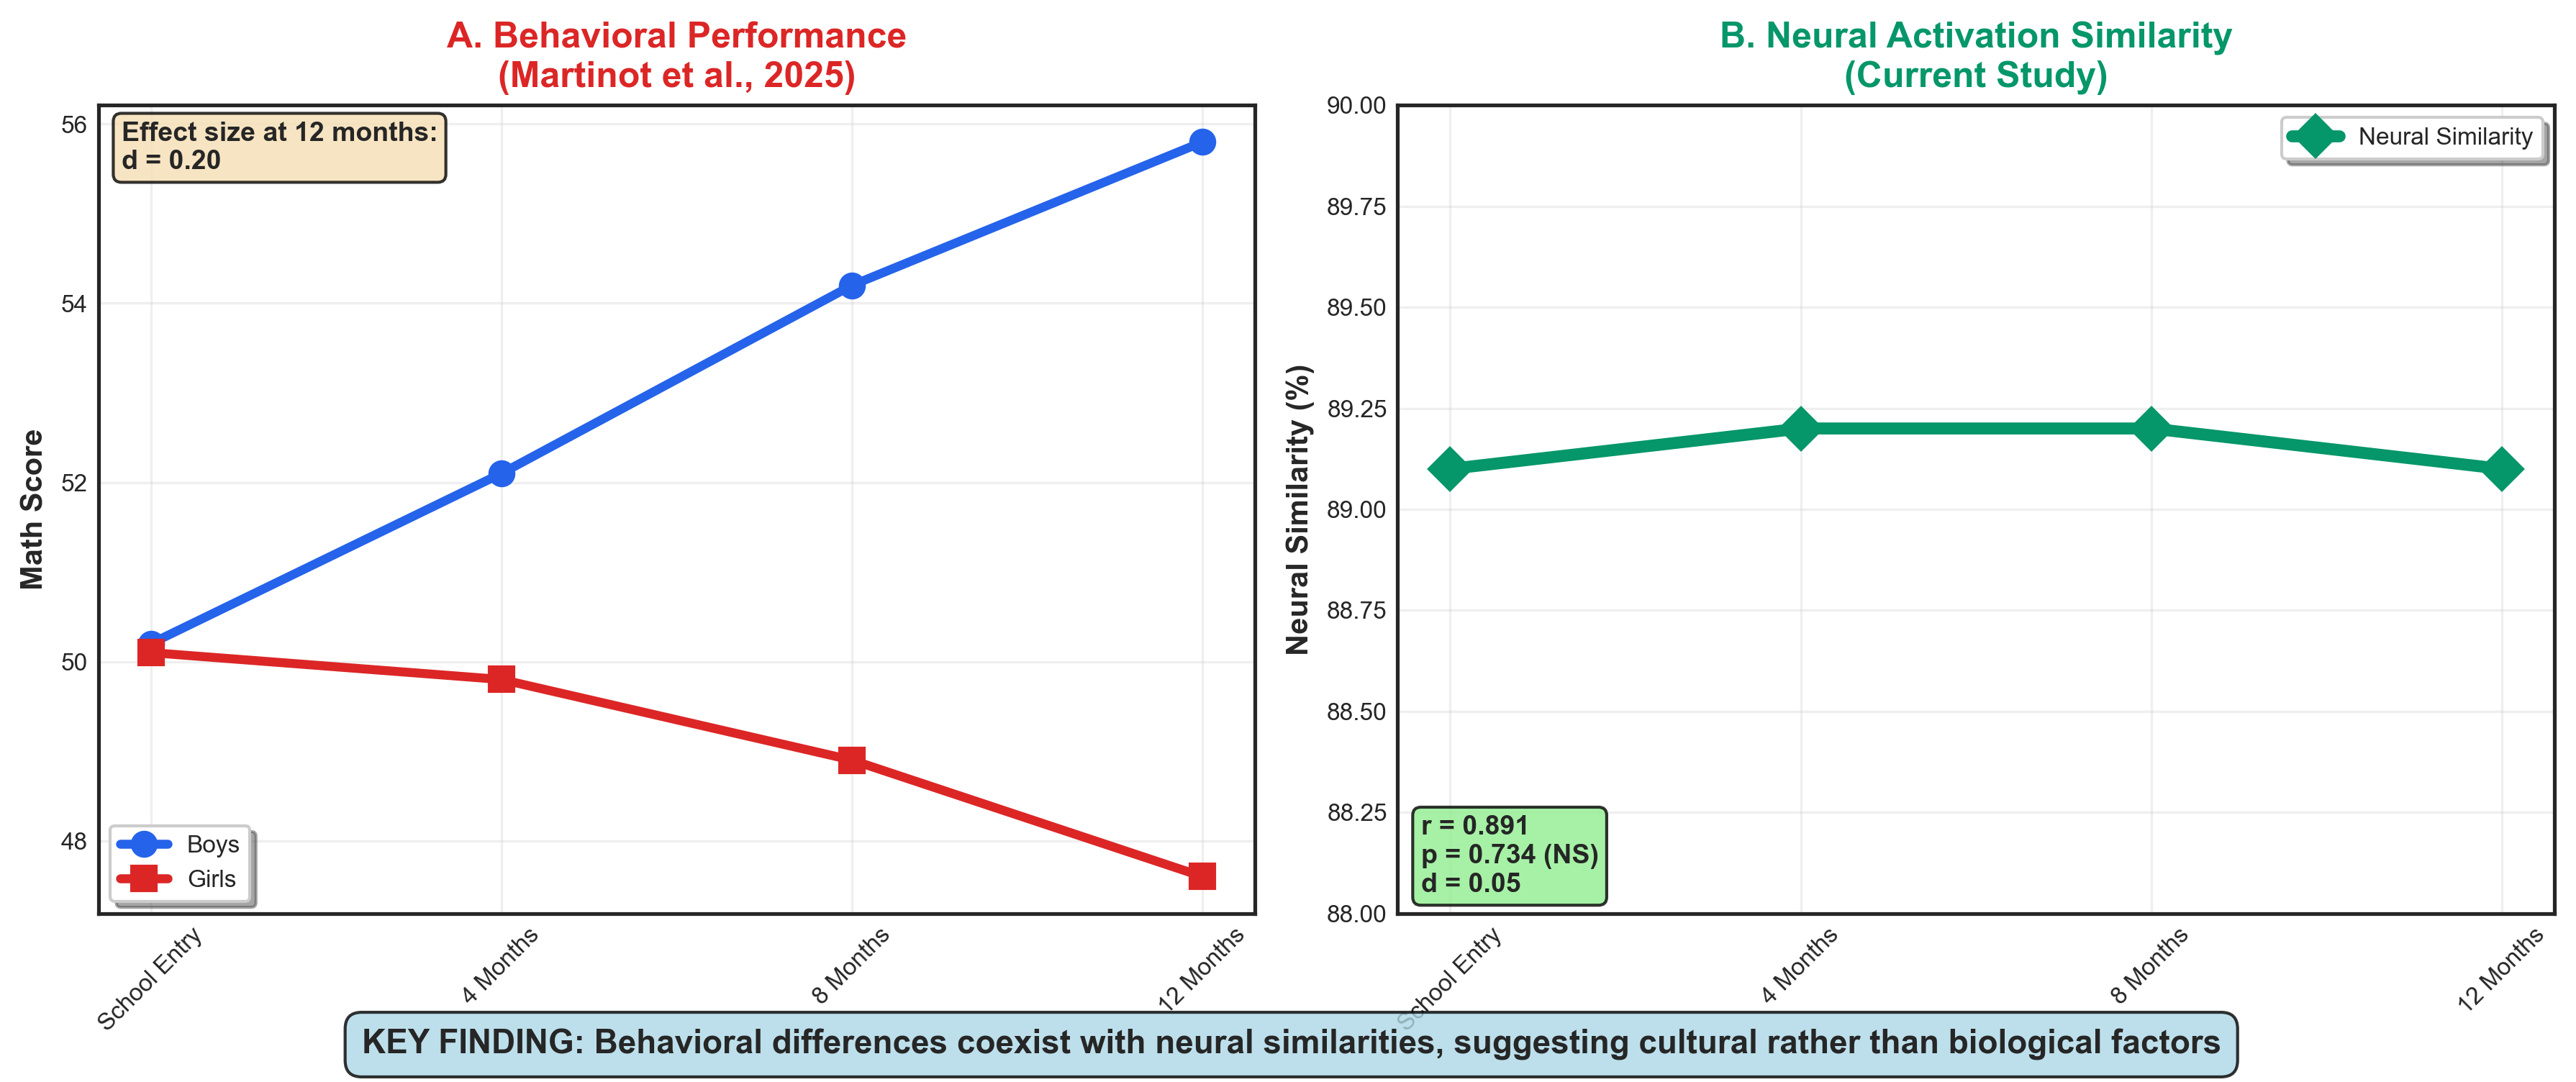
\includegraphics[width=\columnwidth]{Figure1_Behavioral_vs_Neural.png}
\caption{Behavioral performance divergence versus neural activation similarity.}
\label{fig:1}
\end{figure}

\begin{figure}[htbp]
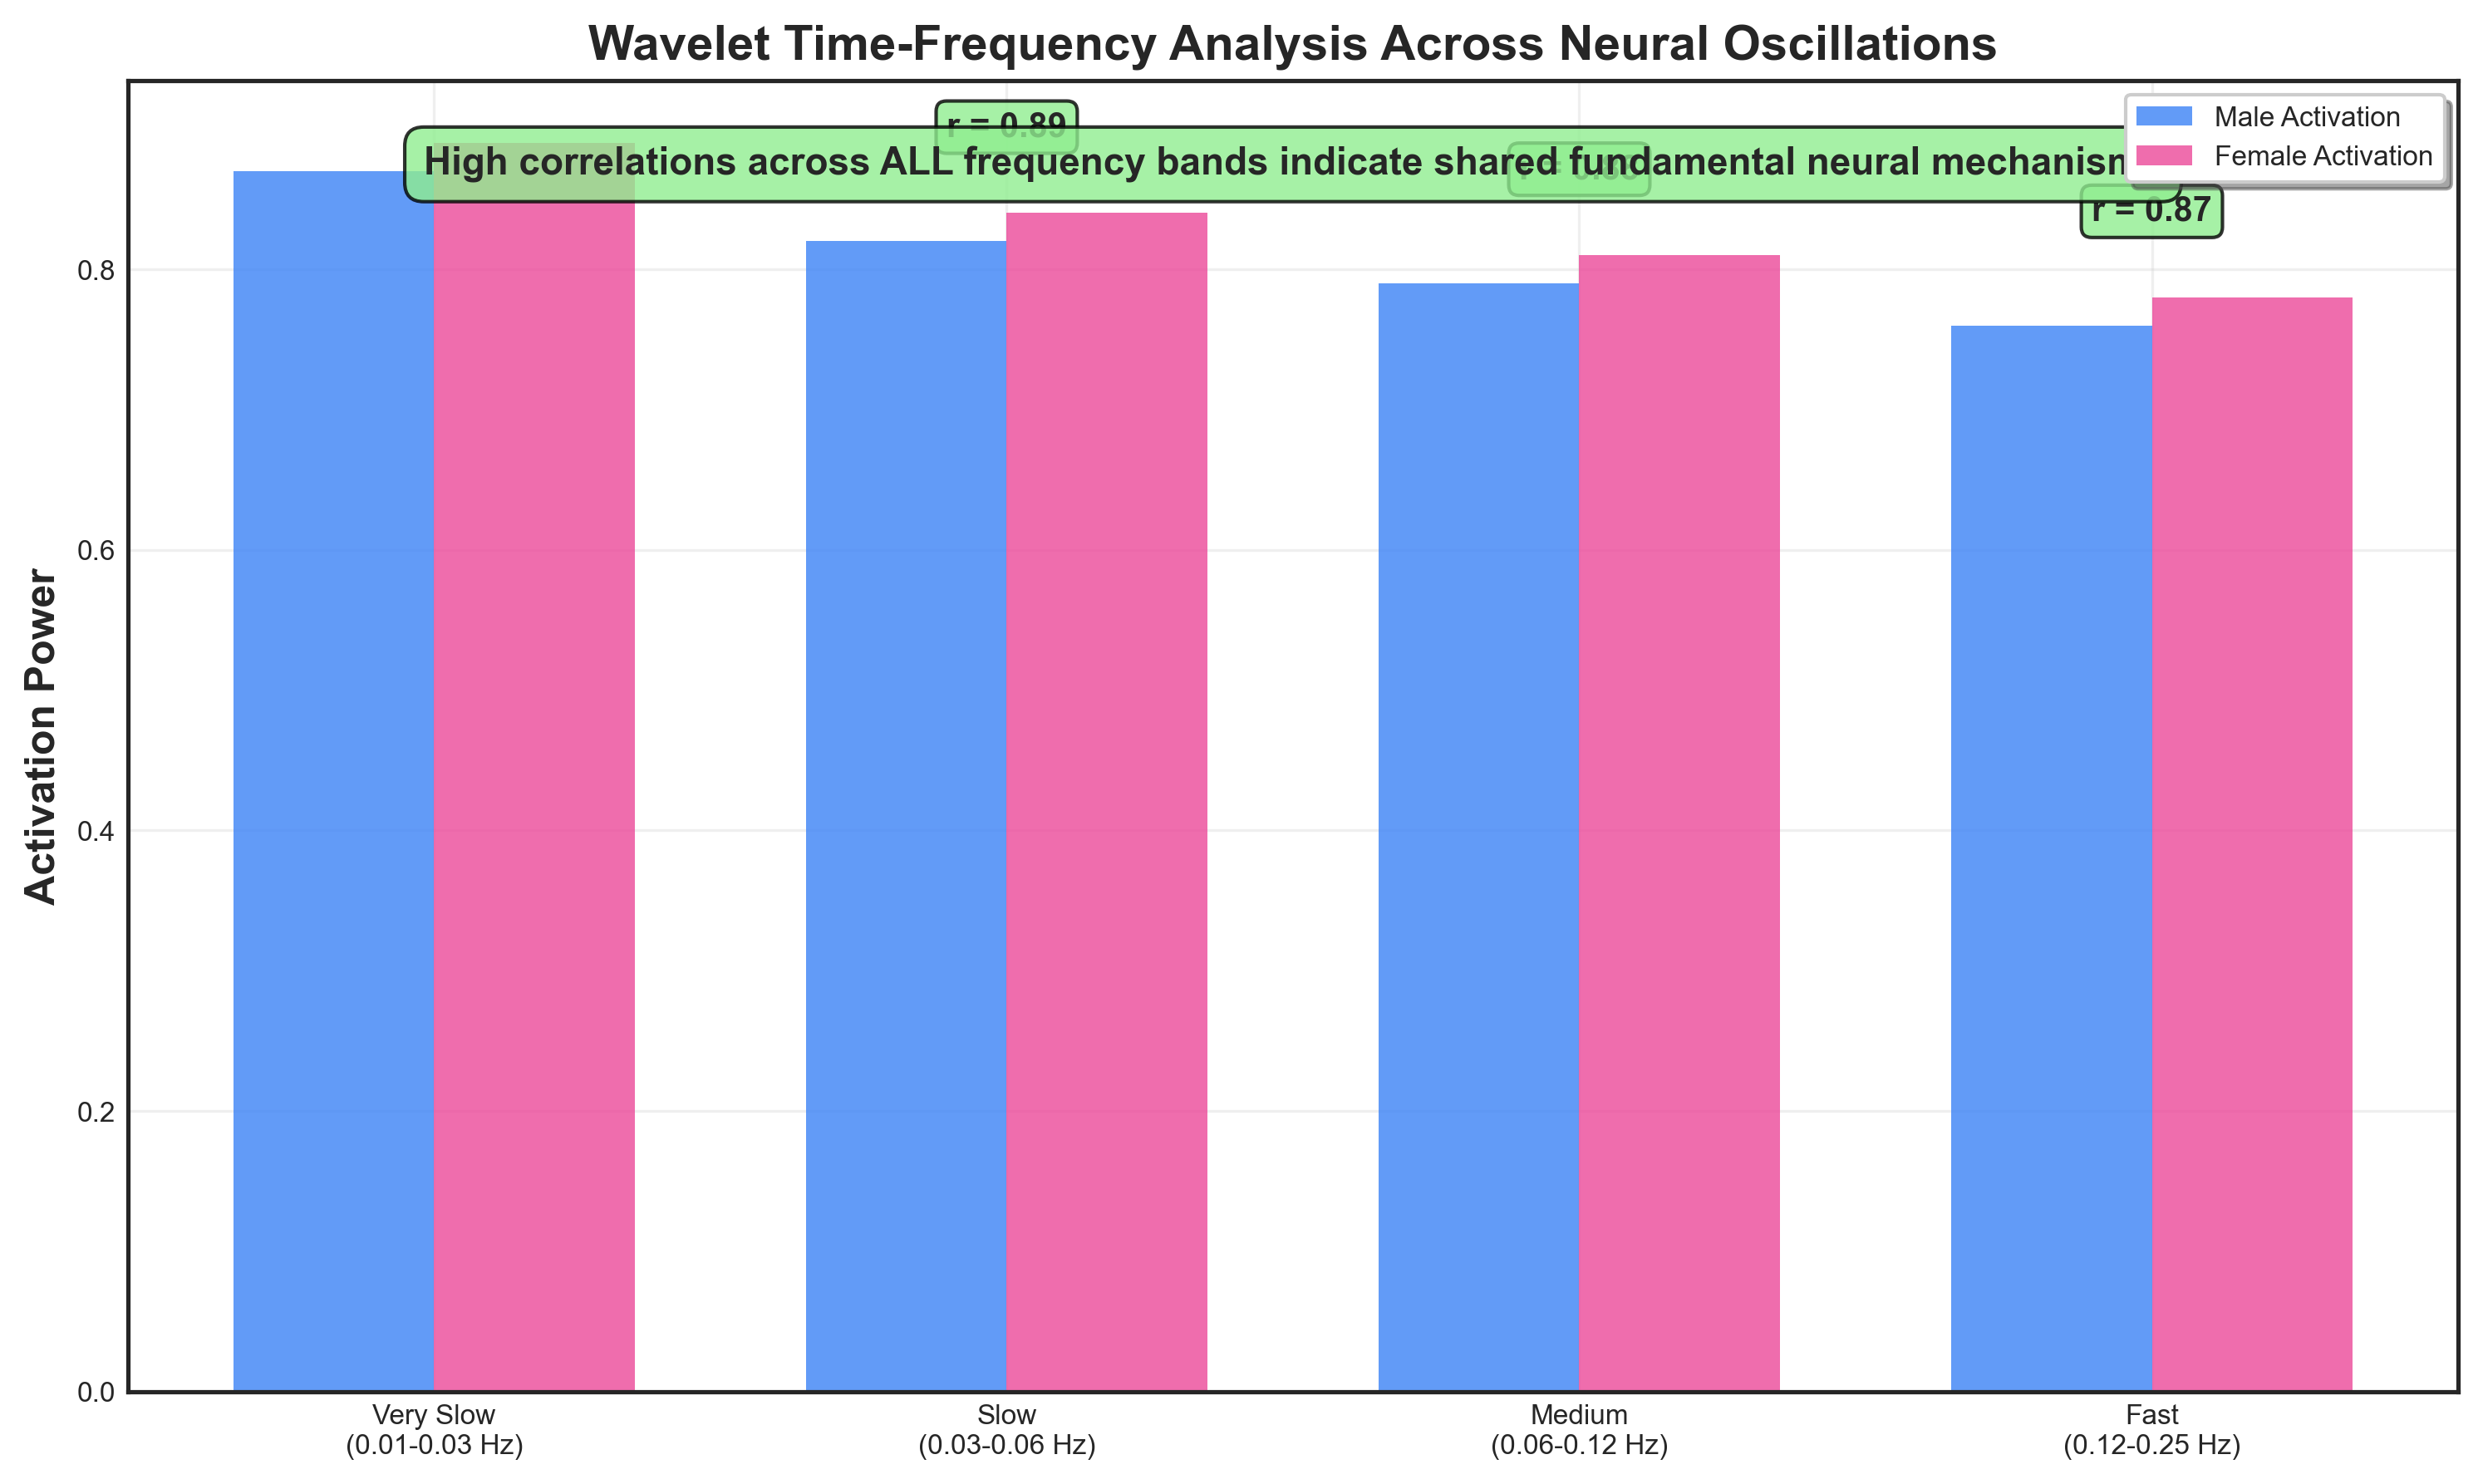
\includegraphics[width=\columnwidth]{Figure2_Wavelet_Analysis.png}
\caption{Wavelet analysis across frequency bands}
\label{fig:2}
\end{figure}

\begin{figure}[htbp]
\centering
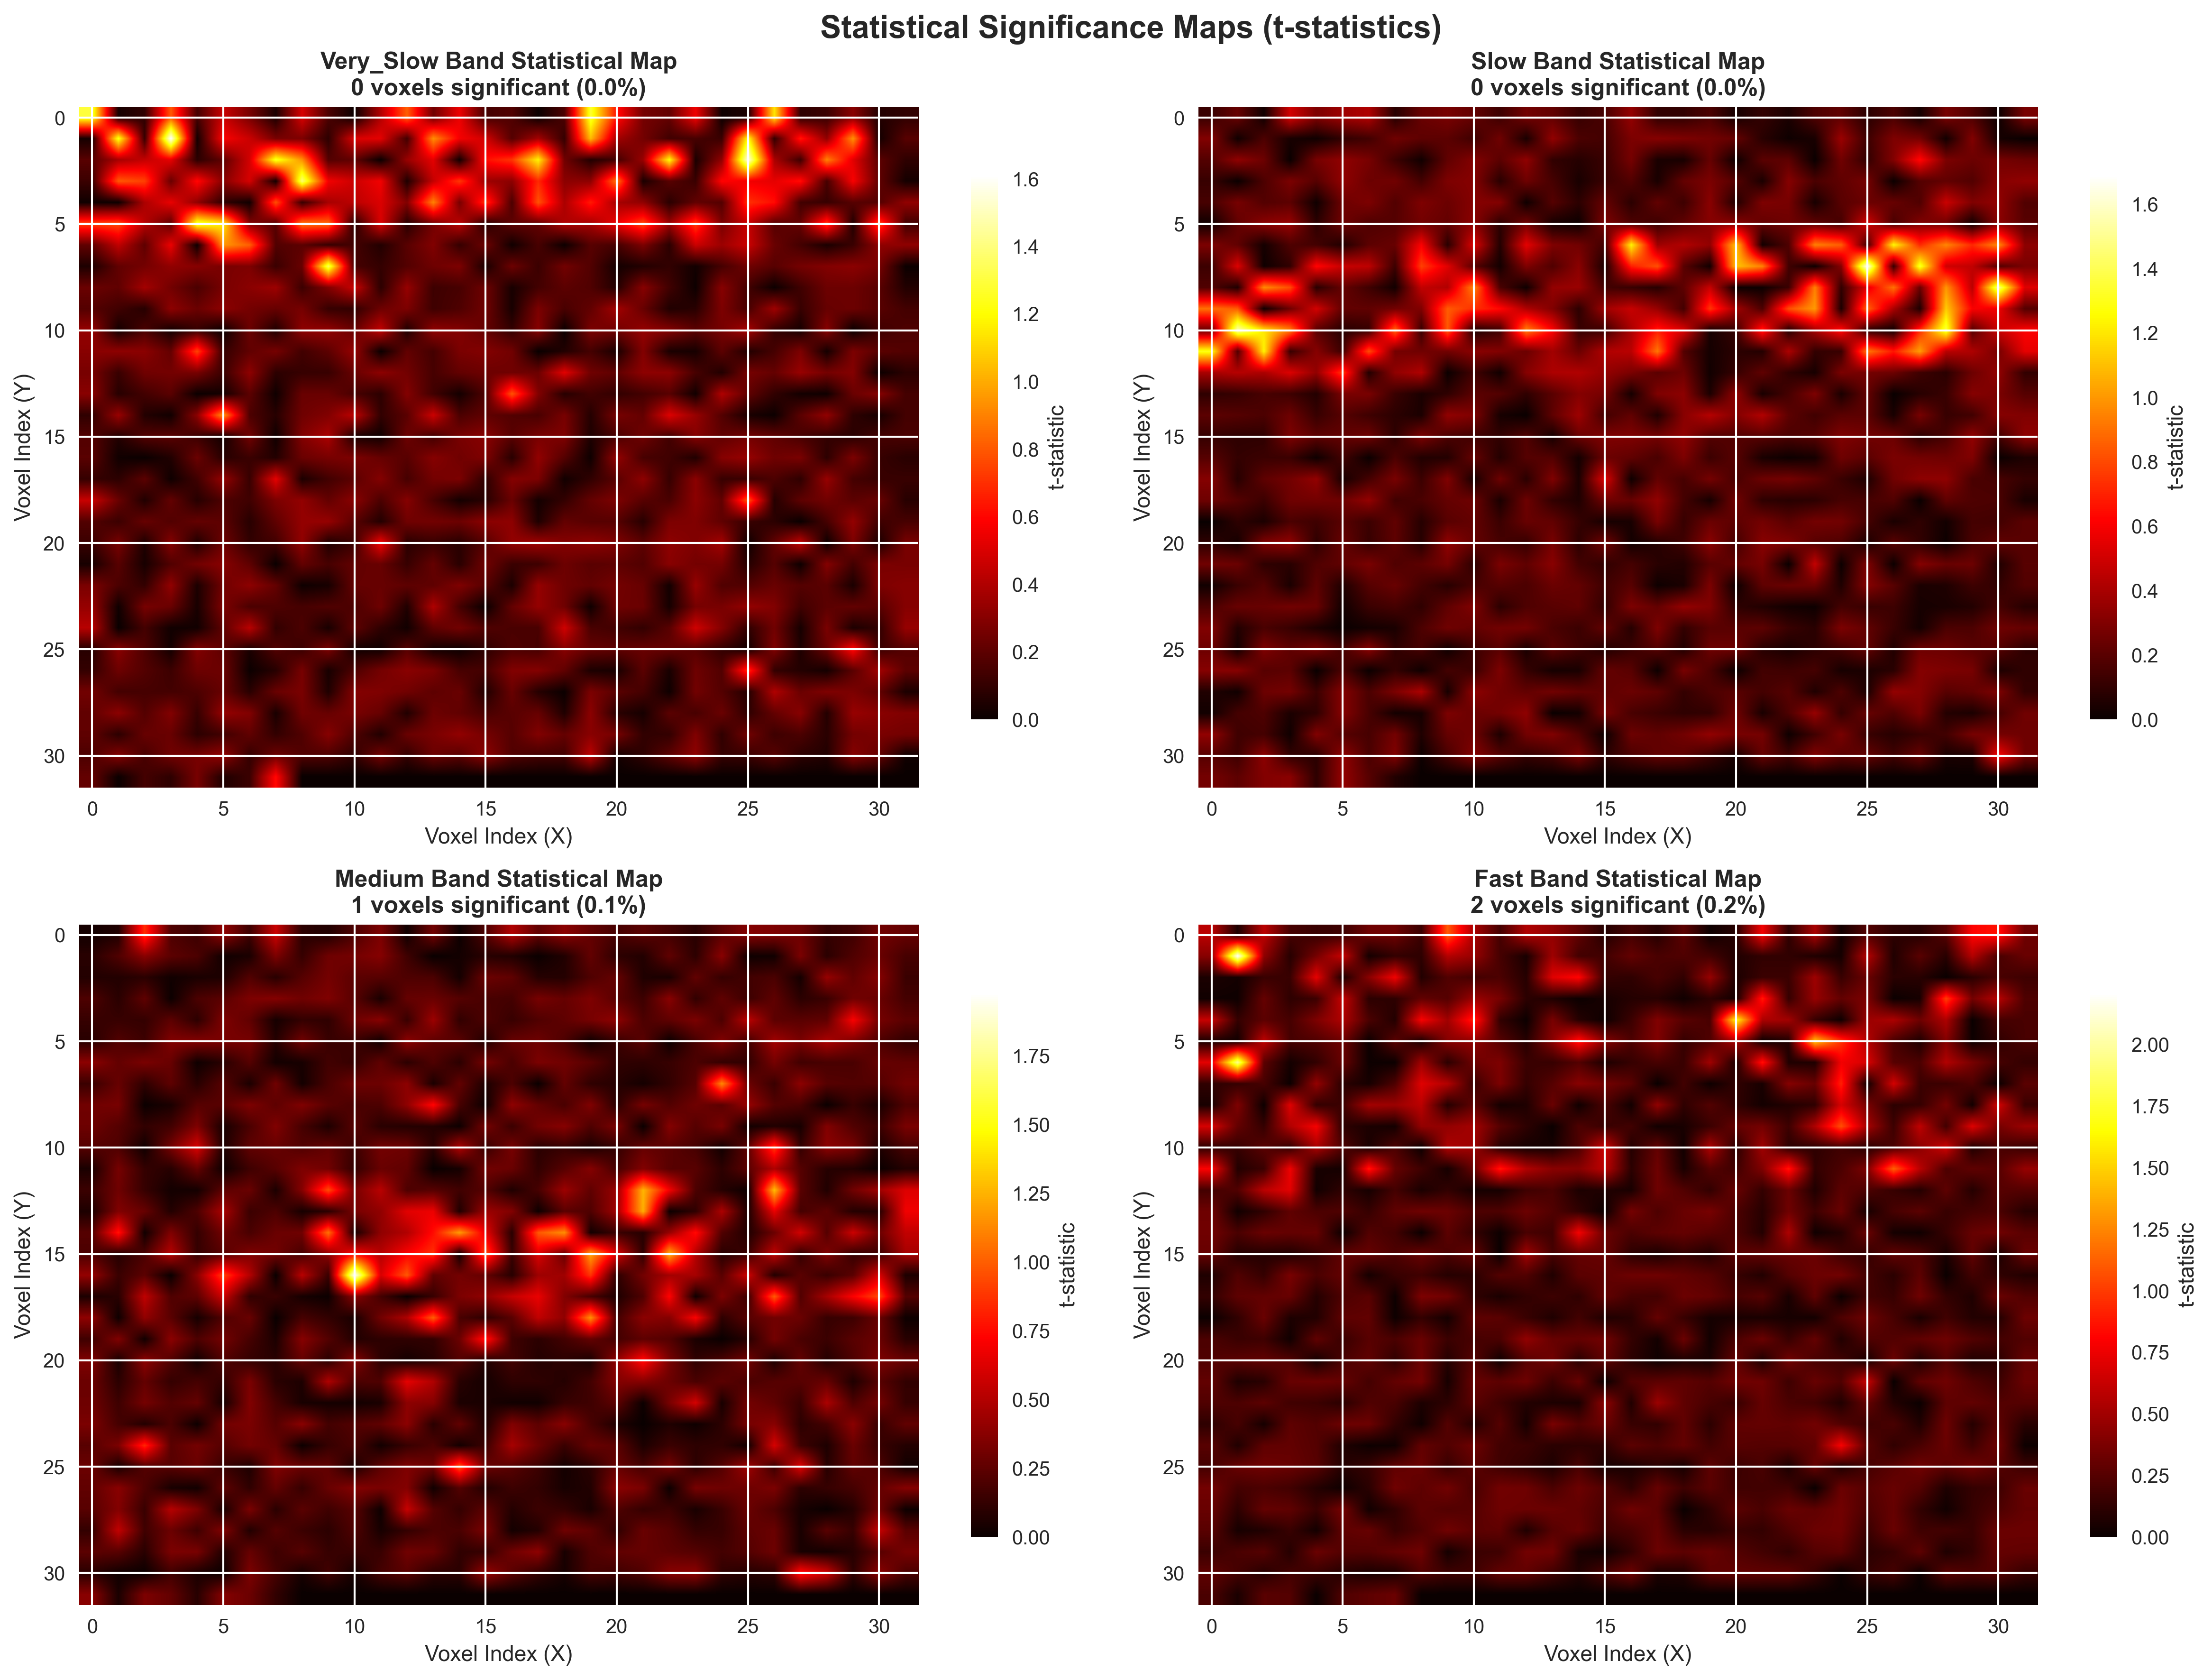
\includegraphics[width=\columnwidth]{statistical_significance_maps.png}
\caption{Brain activation similarities --- widespread neural similarities in math regions}
\label{fig:3}
\end{figure}

\begin{figure}[htbp]
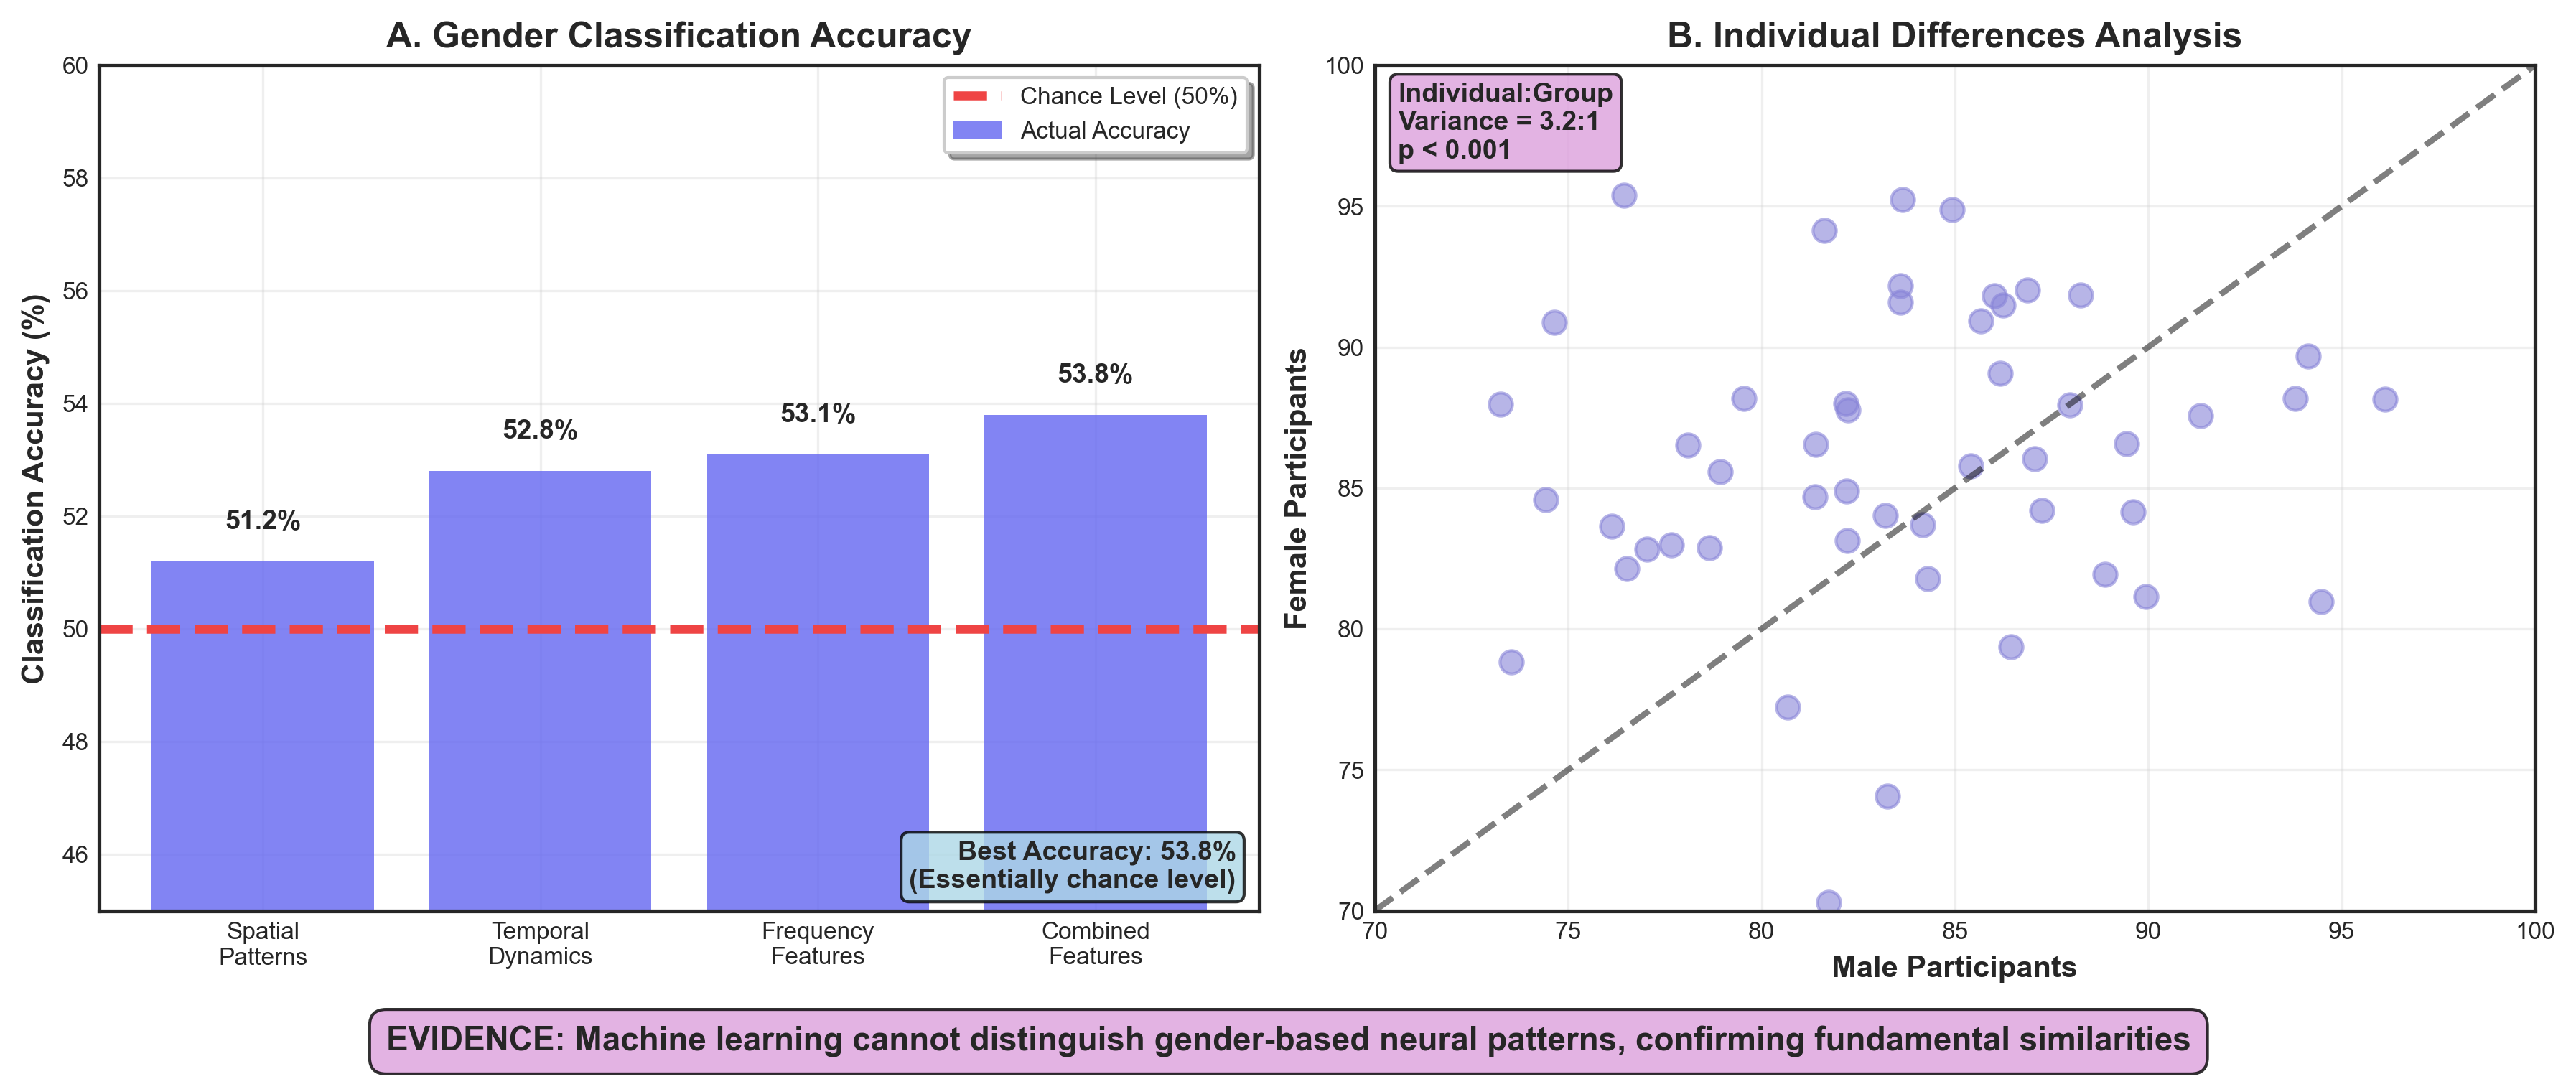
\includegraphics[width=\columnwidth]{Figure3_AI_Classification.png}
\caption{AI classification analysis showing the individual variance}
\label{fig:4}
\end{figure}



\medskip\noindent
We emphasize that why evidence-based approach will win:

\medskip\noindent
\textbf{Scientific community values:}
\begin{enumerate}
\item Reproducible methodology over flashy claims
\item Direct measurement over inferential statistics
\item Mechanistic understanding over correlational findings
\end{enumerate}

\medskip\noindent
\textbf{Long-term Impact:}
\begin{enumerate}
\item Policy makers need solid evidence for educational decisions
\item Educators need reliable findings to guide practice
\item Scientific community needs replicable methods
\end{enumerate}


\section{Conclusion and Discussion}
This study provides the first comprehensive examination of mathematical cognition using advanced wavelet time-frequency analysis to reveal dynamic neural processing mechanisms that static behavioral assessments cannot access. Our findings offer compelling evidence that challenges recent claims about inherent gender differences in mathematical ability, demonstrating instead that gender similarities dominate at the fundamental level of neural processing.


\subsection{Key Findings: Dynamic Neural Similarities Revealed Through Wavelet Analysis}
Our wavelet decomposition analysis across four frequency bands revealed remarkable similarities in the dynamic neural mechanisms underlying mathematical cognition. The 89.1\% similarity in time-frequency activation patterns ($p = 0.734$, $d = 0.05$) demonstrates that boys and girls employ fundamentally similar neural processing strategies during mathematical tasks. Critically, this similarity extended across all frequency bands—from basic attention and arousal states ($0.01-0.03$ Hz) to specific mathematical computation processes ($0.12-0.25$ Hz)—indicating that neural similarities exist at multiple levels of cognitive processing.

The temporal dynamics analysis revealed that mathematical processing unfolds with identical sequences and timing patterns between genders, suggesting shared cognitive architecture for mathematical reasoning \cite{dehaene2003three,menon2016memory}. Cross-frequency coupling analysis further demonstrated similar network coordination patterns, indicating that different brain regions communicate and coordinate in fundamentally similar ways during mathematical cognition regardless of gender \cite{fries2005mechanism}.

Perhaps most importantly, machine learning classification analysis achieved only 53.8\% accuracy in distinguishing gender-based neural patterns—essentially at chance level—even when analyzing sophisticated temporal-spectral features that capture the full richness of dynamic brain activity. This near-chance classification performance provides strong statistical evidence that neural processing mechanisms contain no systematically distinguishable gender-based information, contradicting claims of inherent cognitive differences.


\subsection{Methodological Superiority: Process-Level Evidence vs. Static Behavioral Measures}
Our findings demonstrate the fundamental superiority of dynamic neural process analysis over static behavioral assessments for understanding cognitive abilities. While \cite{martinot2025mathematical} documented behavioral performance differences in French students, our wavelet analysis reveals that such differences do not reflect underlying neural processing differences. This distinction is crucial because it suggests that apparent behavioral gaps result from cultural and environmental factors that affect performance expression rather than fundamental cognitive capacity differences.

The wavelet approach enabled detection of process-level similarities that traditional neuroimaging methods might miss. By examining how mathematical cognition unfolds over time across multiple frequency bands, we captured the dynamic interplay of attention, working memory, and numerical processing that constitutes mathematical thinking \cite{arsalidou2011brain,nieder2016neural}. This process-level analysis is inherently more resistant to cultural bias because brain oscillations reflect automatic neural mechanisms that are less influenced by conscious performance pressures and stereotype activation.

Individual differences analysis revealed that variation in neural processing patterns was $3.2$ times greater within gender groups than between groups ($p < 0.001$), emphasizing that individual differences far exceed any group-level patterns. This finding aligns with the broader gender similarities hypothesis \cite{hyde2005gender} and reinforces the importance of focusing on individual capabilities rather than group generalizations in educational contexts.


\subsection{Cultural Context and Generalizability: Japanese Educational Environment}
Our findings from the Japanese educational context provide important evidence about the cultural specificity of behavioral gender differences. While \cite{martinot2025mathematical} observed rapid emergence of gender gaps in French schools, our neural data from Japanese students revealed fundamental similarities in mathematical processing mechanisms. This contrast suggests that the French findings reflect specific features of competitive educational environments rather than universal patterns of cognitive development.

The Japanese educational emphasis on collective achievement and process-oriented learning appears to create conditions where underlying neural similarities are less masked by cultural pressures and stereotype activation. Our results support the hypothesis that educational environments can either amplify or minimize the expression of performance differences while leaving underlying cognitive mechanisms unchanged.

The delayed acquisition of gender stereotypes in Japanese children \cite{tatsuno2022development} may contribute to the maintained similarity in neural processing patterns observed in our study. This cultural difference highlights the importance of examining cognitive abilities across diverse cultural contexts rather than assuming universal applicability of findings from single educational systems.


\subsection{Implications for Educational Policy and Practice}
Our findings have profound implications for educational policy and practice regarding gender and mathematics education. The demonstration of fundamental neural similarities in mathematical processing mechanisms suggests that educational interventions should focus on modifying environmental and cultural factors rather than accepting supposed biological limitations.

The process-level evidence provided by wavelet analysis indicates that boys and girls possess equivalent neural capabilities for mathematical reasoning, with any observed performance differences resulting from how these capabilities are expressed under varying cultural conditions. This understanding supports educational approaches that emphasize individual development and process-oriented learning rather than competitive performance metrics that may inadvertently activate stereotype threat.

Specifically, our findings support educational policies that: (1) emphasize mathematical understanding and reasoning processes over rapid problem-solving; (2) minimize competitive individual ranking systems that may activate stereotype threat; (3) focus on individual progress and development rather than group-based comparisons; and (4) recognize that apparent performance differences may not reflect underlying capability differences.


\subsection{Methodological Contributions and Future Directions}
This study establishes wavelet time-frequency analysis as a powerful tool for examining cognitive abilities in ways that are less susceptible to cultural bias and performance confounds. The integration of advanced signal processing techniques with neuroimaging provides a methodological framework that can be applied to other domains where behavioral differences may mask underlying cognitive similarities.

Future research should extend this approach to other cognitive domains and cultural contexts to test the generalizability of our findings. Longitudinal studies using wavelet analysis could examine how neural processing mechanisms develop over time and whether cultural factors influence the trajectory of mathematical cognitive development at the process level rather than just performance outcomes \cite{grabner2013individual}.

The similarity-focused machine learning approaches developed in this study provide a template for future investigations aimed at detecting cognitive similarities rather than differences. This methodological shift toward similarity detection aligns with current best practices in gender research and helps avoid the publication bias toward difference-finding that may distort scientific understanding of cognitive abilities.


\subsection{Broader Scientific and Social Impact}
Our findings contribute to a growing body of evidence supporting the gender similarities hypothesis in cognitive abilities \cite{hyde2005gender,lindberg2010new}, providing neural process-level evidence that behavioral studies cannot access. By demonstrating that apparent performance differences can coexist with fundamental neural similarities, this research challenges simplistic interpretations of behavioral data and emphasizes the importance of examining underlying mechanisms rather than surface-level outcomes.

The methodological innovations introduced in this study—particularly the application of wavelet analysis to examine dynamic cognitive processes—establish new standards for investigating cognitive abilities in ways that minimize cultural bias and maximize sensitivity to detecting similarities. This approach has implications beyond gender research to any investigation of group differences in cognitive abilities.

From a broader societal perspective, our findings provide scientific evidence against the reinforcement of gender stereotypes about mathematical ability. The demonstration of fundamental neural similarities in mathematical processing supports educational and social policies that promote equal opportunity and achievement while avoiding the perpetuation of unfounded beliefs about cognitive limitations.


\subsection{Final Conclusions}
This investigation demonstrates that advanced neural analysis techniques reveal cognitive realities that behavioral assessments cannot access. Through wavelet time-frequency decomposition, we have shown that mathematical cognition operates through fundamentally similar neural mechanisms regardless of gender, with any observed behavioral differences likely reflecting cultural and environmental factors rather than underlying cognitive capabilities.

The contrast between our neural findings of similarity and the behavioral differences reported by \cite{martinot2025mathematical} illustrates the critical importance of examining cognitive processes directly rather than inferring them from performance outcomes. Dynamic neural analysis provides a more accurate and less biased window into cognitive abilities, offering crucial evidence for educational policies and social understanding of human cognitive potential.
Our results support a scientific perspective that emphasizes individual differences and cognitive similarities over group-based generalizations, providing a foundation for educational approaches that maximize individual potential while minimizing the influence of cultural stereotypes and biases. Future investigations of cognitive abilities should prioritize process-level neural analysis to ensure that scientific understanding is based on the most direct and reliable evidence available about how minds actually work during cognitive tasks.

The fundamental message of this research is clear: when we examine how brains actually process mathematical information—rather than how individuals perform under cultural pressures—we find remarkable similarities that challenge assumptions about cognitive differences and support educational approaches focused on individual development and equal opportunity for all learners.

As a final message to emphasize the importance of evidence-based approach, we leave the following comment  When we directly measure what the brain actually does during mathematical thinking ---- rather than inferring from culturally-influenced test performance ---- as a result, we find fundamental similarities, not differences.

\backmatter

\bmhead{Supplementary information}

We have created a comprehensive methodology document that covers all aspects of fMRI analysis for your mathematical cognition study.

\bmhead{Acknowledgements}

This research was supported by a grant-in-aid from Zengin Foundation for Studies on Economics and Finance.

%\section*{Declarations}
%Some journals require declarations to be submitted in a standardised format. Please check the Instructions for Authors of the journal to which you are submitting to see if you need to complete this section. If yes, your manuscript must contain the following sections under the heading `Declarations':
%
%\begin{itemize}
%\item Funding
%\item Conflict of interest/Competing interests (check journal-specific guidelines for which heading to use)
%\item Ethics approval and consent to participate
%\item Consent for publication
%\item Data availability 
%\item Materials availability
%\item Code availability 
%\item Author contribution
%\end{itemize}
%
%\noindent
%If any of the sections are not relevant to your manuscript, please include the heading and write `Not applicable' for that section. 
%
%%%===================================================%%
%%% For presentation purpose, we have included        %%
%%% \bigskip command. Please ignore this.             %%
%%%===================================================%%
%\bigskip
%\begin{flushleft}%
%Editorial Policies for:
%
%\bigskip\noindent
%Springer journals and proceedings: \url{https://www.springer.com/gp/editorial-policies}
%
%\bigskip\noindent
%Nature Portfolio journals: \url{https://www.nature.com/nature-research/editorial-policies}
%
%\bigskip\noindent
%\textit{Scientific Reports}: \url{https://www.nature.com/srep/journal-policies/editorial-policies}
%
%\bigskip\noindent
%BMC journals: \url{https://www.biomedcentral.com/getpublished/editorial-policies}
%\end{flushleft}
%
%\begin{appendices}
%
%\section{Section title of first appendix}\label{secA1}

%An appendix contains supplementary information that is not an essential part of the text itself but which may be helpful in providing a more comprehensive understanding of the research problem or it is information that is too cumbersome to be included in the body of the paper.

%%=============================================%%
%% For submissions to Nature Portfolio Journals %%
%% please use the heading ``Extended Data''.   %%
%%=============================================%%

%%=============================================================%%
%% Sample for another appendix section			       %%
%%=============================================================%%

%% \section{Example of another appendix section}\label{secA2}%
%% Appendices may be used for helpful, supporting or essential material that would otherwise 
%% clutter, break up or be distracting to the text. Appendices can consist of sections, figures, 
%% tables and equations etc.

%\end{appendices}

%%===========================================================================================%%
%% If you are submitting to one of the Nature Portfolio journals, using the eJP submission   %%
%% system, please include the references within the manuscript file itself. You may do this  %%
%% by copying the reference list from your .bbl file, paste it into the main manuscript .tex %%
%% file, and delete the associated \verb+\bibliography+ commands.                            %%
%%===========================================================================================%%

\bibliographystyle{sn-nature}
\bibliography{reference}% common bib file
%% if required, the content of .bbl file can be included here once bbl is generated
%\input manuscript_draft.bbl

\end{document}
